% =====================================================================
%  Training_and_Evaluation_Explained.tex
%  How the models were trained, which dataset each model used, how
%  accuracy / precision / recall / confusion matrix are calculated (with
%  worked examples from our own results), example images, and where each
%  item appears in the IEEE paper.
%  Build: tectonic Training_and_Evaluation_Explained.tex
% =====================================================================
\documentclass[10.5pt,a4paper]{article}
% =====================================================================
%  report_preamble.tex -- shared preamble for the stand-alone
%  Datasets and Algorithms reports (article class, A4).
% =====================================================================
\usepackage[T1]{fontenc}
\usepackage[utf8]{inputenc}
\usepackage{mathptmx}
\usepackage[a4paper,margin=2cm]{geometry}
\usepackage{amsmath,amssymb}
\usepackage{graphicx,xcolor}
\usepackage{tikz,pgfplots}
\pgfplotsset{compat=1.18}
\usetikzlibrary{positioning,arrows.meta,calc}
\usepackage{booktabs,array,multirow,tabularx,longtable}
\usepackage{pifont}
\providecommand{\checkmark}{\ding{51}}
\usepackage{enumitem}
\setlist{itemsep=1pt,topsep=3pt,parsep=0pt}
\usepackage[font=small,labelfont=bf]{caption}
\usepackage{float}
\usepackage{cite}
\usepackage{url}
\usepackage[colorlinks=true,linkcolor=hcBlue,citecolor=hcBlue,urlcolor=hcTeal]{hyperref}
\usepackage{titlesec}
\titleformat{\section}{\large\bfseries\color{hcBlue}}{\thesection}{0.6em}{}
\titleformat{\subsection}{\normalsize\bfseries}{\thesubsection}{0.6em}{}
\setlength{\parskip}{3pt}

% ---- Palette (colour-blind friendly) ----------------------------------
\definecolor{hcBlue}{HTML}{2166AC}
\definecolor{hcTeal}{HTML}{1B9E77}
\definecolor{hcOrange}{HTML}{D95F02}
\definecolor{hcPurple}{HTML}{7570B3}
\definecolor{hcRed}{HTML}{B2182B}
\definecolor{hcGray}{HTML}{6E6E6E}
\definecolor{boxBg}{HTML}{EEF3FA}

\pgfplotsset{
  hcaxis/.style={
    tick align=outside, tick pos=left, grid=major,
    major grid style={line width=0.2pt,draw=gray!30},
    axis line style={draw=gray!55},
    label style={font=\footnotesize},
    tick label style={font=\scriptsize},
    legend style={font=\scriptsize,draw=gray!40,fill=white,rounded corners=1pt},
    every node near coord/.append style={font=\tiny},
  }
}

\newcolumntype{L}[1]{>{\raggedright\arraybackslash}p{#1}}
\newcolumntype{Y}{>{\raggedright\arraybackslash}X}

% Highlight box for key take-aways
\newcommand{\keybox}[1]{%
  \par\smallskip\noindent\colorbox{boxBg}{\parbox{\dimexpr\linewidth-2\fboxsep}{\small #1}}\par\smallskip}

\setlength{\parindent}{0pt}
\newcommand{\inpaper}[1]{\par\smallskip{\small\color{hcTeal}\textbf{In the paper:} #1}\par\smallskip}

\title{\color{hcBlue}\bfseries How We Trained and Evaluated the Models\\[4pt]
\large Accuracy, Precision, Confusion Matrix --- with Real Examples from Our Project}
\author{Project: Skin Cancer Detection Using Deep Learning}
\date{}

\begin{document}
\maketitle
\vspace{-8mm}

\keybox{\textbf{In one sentence:} we trained three models (EfficientNetV2-S,
ConvNeXt-T, Swin-T) on the same 18{,}076 ISIC~2019 training images,
combined their answers by averaging, and tested them on 3{,}596 ISIC~2019
images and 2{,}298 PAD-UFES-20 phone photos that they had never seen. The
combined model classified \textbf{2{,}803 of 3{,}596} test images correctly
(\textbf{77.95\% accuracy}) with \textbf{68.67\% precision} (macro average).}

\tableofcontents

% =====================================================================
\section{Which Dataset Was Used by Which Model}
All three models were trained on \textbf{exactly the same data}. This
is important: it makes the comparison between the models fair, and it
means the ensemble's improvement comes from combining the models, not
from extra data.

\begin{center}
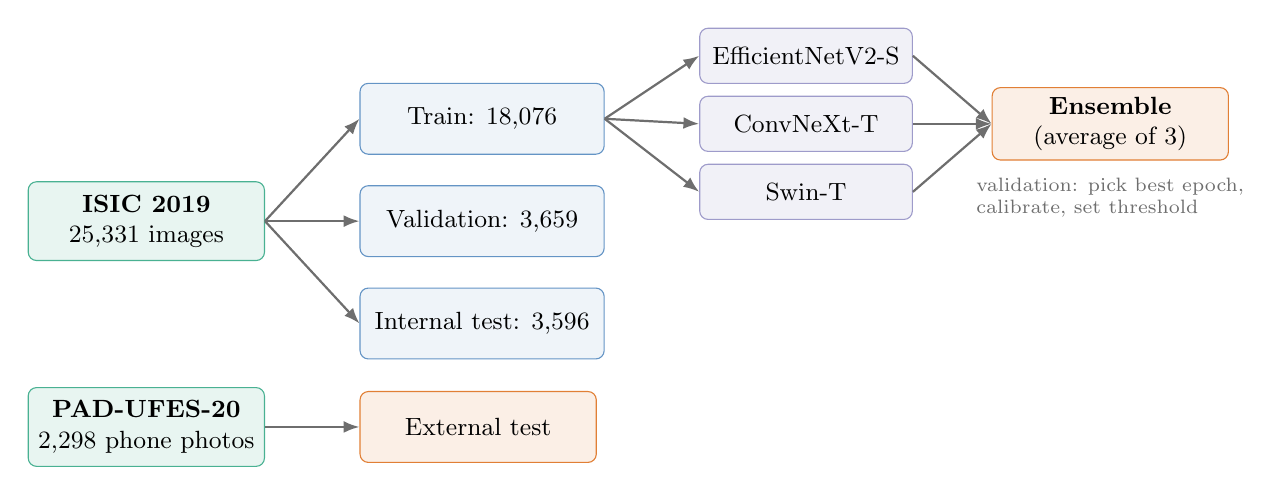
\begin{tikzpicture}[font=\small, node distance=4mm and 9mm,
  ds/.style={draw=hcTeal!80,fill=hcTeal!10,rounded corners=3pt,minimum width=30mm,minimum height=10mm,align=center},
  sp/.style={draw=hcBlue!70,fill=hcBlue!7,rounded corners=3pt,minimum width=31mm,minimum height=9mm,align=center},
  md/.style={draw=hcPurple!70,fill=hcPurple!10,rounded corners=3pt,minimum width=27mm,minimum height=7mm,align=center},
  ot/.style={draw=hcOrange!80,fill=hcOrange!10,rounded corners=3pt,minimum width=30mm,minimum height=9mm,align=center},
  fl/.style={-{Latex[length=2mm]},draw=hcGray,thick}]
\node[ds] (isic) {\textbf{ISIC 2019}\\25{,}331 images};
\node[sp,right=12mm of isic,yshift=13mm] (tr) {Train: 18{,}076};
\node[sp,right=12mm of isic] (va) {Validation: 3{,}659};
\node[sp,right=12mm of isic,yshift=-13mm] (te) {Internal test: 3{,}596};
\node[md,right=12mm of tr,yshift=8mm] (m1) {EfficientNetV2-S};
\node[md,below=1.5mm of m1] (m2) {ConvNeXt-T};
\node[md,below=1.5mm of m2] (m3) {Swin-T};
\node[ot,right=10mm of m2] (ens) {\textbf{Ensemble}\\(average of 3)};
\node[ds,below=16mm of isic] (pad) {\textbf{PAD-UFES-20}\\2{,}298 phone photos};
\node[ot,right=12mm of pad] (ext) {External test};
\draw[fl] (isic.east)--(tr.west); \draw[fl] (isic.east)--(va.west); \draw[fl] (isic.east)--(te.west);
\draw[fl] (tr.east)--(m1.west); \draw[fl] (tr.east)--(m2.west); \draw[fl] (tr.east)--(m3.west);
\draw[fl] (m1.east)--(ens.west); \draw[fl] (m2.east)--(ens.west); \draw[fl] (m3.east)--(ens.west);
\draw[fl] (pad)--(ext);
\node[font=\scriptsize,text=hcGray,align=left,below=1mm of ens] {validation: pick best epoch,\\calibrate, set threshold};
\end{tikzpicture}
\end{center}

\begin{tabularx}{\linewidth}{@{}L{3.1cm} L{3.4cm} L{3.4cm} Y@{}}
\toprule
\textbf{Model} & \textbf{Trained on} & \textbf{Tuned on} & \textbf{Tested on} \\
\midrule
EfficientNetV2-S (CNN) & ISIC 2019 train, 18{,}076 & ISIC 2019 validation, 3{,}659 & ISIC 2019 test (3{,}596) + PAD-UFES-20 (2{,}298) \\
ConvNeXt-T (CNN) & same 18{,}076 & same 3{,}659 & same test sets \\
Swin-T (transformer) & same 18{,}076 & same 3{,}659 & same test sets \\
Ensemble (ours) & no extra training: averages the 3 models & temperatures, weights, threshold & same test sets \\
\bottomrule
\end{tabularx}

\textbf{Why this split?} Photos of the same mole were always kept in the
same part (train, validation, or test), and 344 groups of near-identical
photos were merged, so the models are never tested on a mole they have
already seen. PAD-UFES-20 was \emph{never} used for training; it checks
whether the models work on a different kind of photo.

\inpaper{Section III (Datasets), Table II (``Used'' rows), Section V-A
(Leakage-free protocol).}

% =====================================================================
\section{How We Trained the Models}
\begin{enumerate}
  \item \textbf{Prepare images.} Every photo was resized (shorter side 256
        pixels). During training a random $224\times224$ crop is taken,
        flipped, rotated, and colour-changed slightly (\emph{augmentation}),
        so the model sees a slightly different version every time.
  \item \textbf{Start from pre-trained models.} Each model had already
        learned general images (ImageNet-21k). We replaced its last layer
        with a new one for our 8 skin classes. This is \emph{transfer
        learning}.
  \item \textbf{Train with focal loss.} The model looks at a batch of 32
        photos, predicts, and the \emph{focal loss} measures how wrong it was
        (rare classes such as SCC get extra weight). The AdamW optimizer then
        adjusts the model's weights a little. One pass over all 18{,}076
        photos is one \emph{epoch}.
  \item \textbf{Check after every epoch.} After each epoch the model is
        scored on the 3{,}659 validation photos (balanced accuracy). The best
        epoch is saved; training stops after 20 epochs or after 6 epochs
        without improvement (\emph{early stopping}).
  \item \textbf{Combine.} Each model's confidence is calibrated
        (\emph{temperature scaling}); then the three probability lists are
        averaged (\emph{soft voting}).
  \item \textbf{Test once.} Only at the end are the test sets used.
\end{enumerate}

\begin{tabularx}{\linewidth}{@{}l c c c Y@{}}
\toprule
\textbf{Model} & \textbf{Epochs run} & \textbf{Best epoch} & \textbf{Best val.\ BA} & \textbf{Training time (RTX 3060 laptop)} \\
\midrule
EfficientNetV2-S & 20 & 19 & 64.16\% & 43 min \\
ConvNeXt-T & 20 & 17 & 64.61\% & 49 min \\
Swin-T & 11 (early stop) & 5 & 63.05\% & 36 min \\
\bottomrule
\end{tabularx}

\begin{figure}[H]
\centering
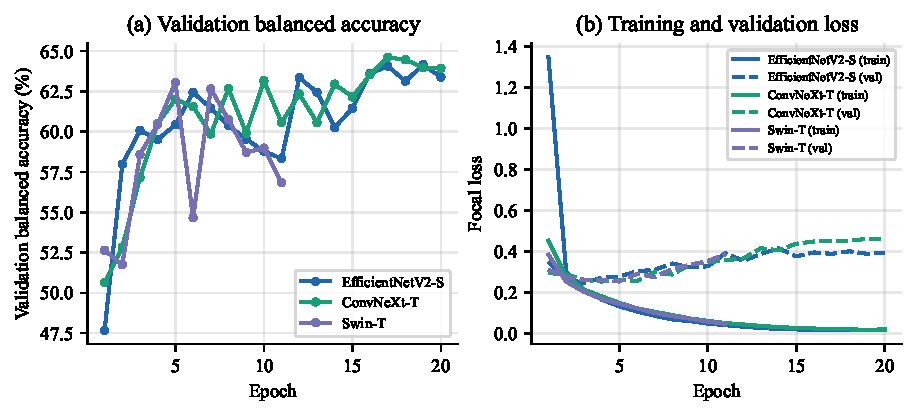
\includegraphics[width=0.95\linewidth]{figures/fig_training_curves.pdf}
\caption{Real training curves. Left: validation balanced accuracy per epoch. Right: loss (solid = training, dashed = validation).}
\end{figure}

\inpaper{Section IV-I (Training procedure), Algorithm 1, Table III
(settings), Fig.~4 (training curves), Section VI-A.}

% =====================================================================
\section{How One Prediction Is Made (Real Example)}
\begin{minipage}{0.30\linewidth}
\centering
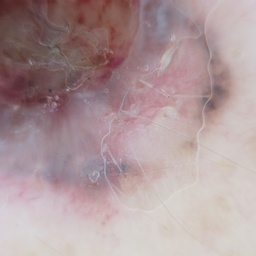
\includegraphics[width=\linewidth]{figures/example_test_2188.jpg}\\
{\small Test image ISIC\_0057417\\ true diagnosis: \textbf{melanoma}}
\end{minipage}\hfill
\begin{minipage}{0.66\linewidth}
\small
\begin{tabular}{@{}l c c c l@{}}
\toprule
\textbf{Model} & \textbf{MEL} & \textbf{BCC} & \textbf{SCC} & \textbf{Answer} \\
\midrule
EfficientNetV2-S & 27.2\% & 47.9\% & 21.4\% & BCC (wrong) \\
ConvNeXt-T & 48.2\% & 49.1\% & 0.2\% & BCC (wrong) \\
Swin-T & 78.4\% & 13.8\% & 4.8\% & MEL (right) \\
\midrule
\textbf{Ensemble} & \textbf{51.3\%} & 36.9\% & 8.8\% & \textbf{MEL (right)} \\
\bottomrule
\end{tabular}\\[4pt]
Each model gives a probability for all 8 classes (three shown). The
ensemble averages them, e.g.\ for melanoma
$(27.2+48.2+78.4)/3=51.3\%$, and picks the highest. Two models alone
were wrong, but the combined answer is right.
\end{minipage}

\inpaper{Equation (4) in Section IV-G (Calibrated ensemble).}

% =====================================================================
\section{The Confusion Matrix}
A confusion matrix counts, for every true class (rows), what the model
predicted (columns). The \textbf{diagonal} (top-left to bottom-right) is
correct; everything else is a mistake.

\begin{figure}[H]
\centering
\begin{minipage}{0.56\linewidth}\centering
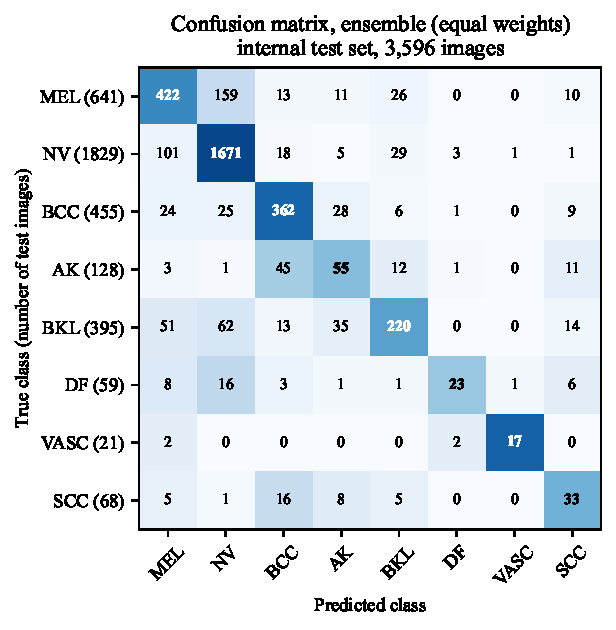
\includegraphics[width=\linewidth]{figures/fig_cm_counts.pdf}
\end{minipage}\hfill
\begin{minipage}{0.42\linewidth}\centering
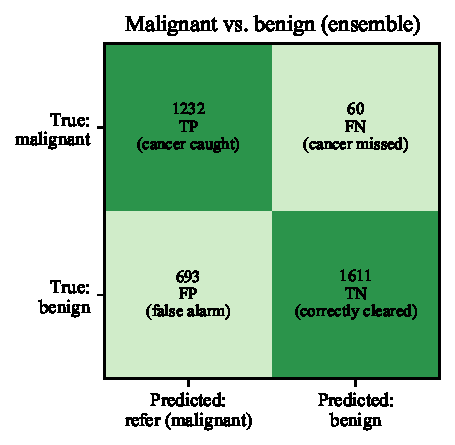
\includegraphics[width=\linewidth]{figures/fig_cm_binary.pdf}
\end{minipage}
\caption{Left: 8-class confusion matrix of the ensemble on the 3{,}596 internal test images (counts). Right: the same predictions as a 2$\times$2 matrix ``malignant (MEL, BCC, SCC, AK) vs.\ benign'' at the referral threshold.}
\end{figure}

\textbf{How to read it:} the melanoma row says that of the 641 real
melanomas, \textbf{422} were predicted as melanoma (correct), 159 as nevus,
26 as benign keratosis, and so on. The melanoma \emph{column} says that
the model predicted ``melanoma'' 616 times in total, and 422 of those
were real melanomas.

\inpaper{Fig.~6 (8-class confusion matrix) in Section VI-C.}

% =====================================================================
\section{How Each Metric Is Calculated (with Our Numbers)}
For one class: \textbf{TP} = true positive (correctly found), \textbf{FP}
= false positive (wrongly predicted as this class), \textbf{FN} = false
negative (this class but missed), \textbf{TN} = true negative.

\renewcommand{\arraystretch}{1.5}
\begin{tabularx}{\linewidth}{@{}L{2.6cm} L{4.3cm} Y@{}}
\toprule
\textbf{Metric} & \textbf{Formula} & \textbf{Worked example from our confusion matrix} \\
\midrule
\textbf{Accuracy} & $\dfrac{\text{correct predictions}}{\text{all images}}$ & Diagonal sum $=422+1671+362+55+220+23+17+33=2803$; $2803/3596=\mathbf{77.95\%}$ \\
\textbf{Precision} (MEL) & $\dfrac{TP}{TP+FP}$ = ``when it says melanoma, how often is it right?'' & $422/616=\mathbf{68.5\%}$ (616 = melanoma column) \\
\textbf{Recall / sensitivity} (MEL) & $\dfrac{TP}{TP+FN}$ = ``of all real melanomas, how many were found?'' & $422/641=\mathbf{65.8\%}$ (641 = melanoma row) \\
\textbf{F1-score} (MEL) & $\dfrac{2\cdot P\cdot R}{P+R}$ & $2\cdot0.685\cdot0.658/(0.685+0.658)=\mathbf{67.1\%}$ \\
\textbf{Macro precision} & average of the 8 class precisions & $(68.5+86.4+77.0+38.5+73.6+76.7+89.5+39.3)/8=\mathbf{68.7\%}$ \\
\textbf{Balanced accuracy} & average of the 8 class recalls & $(65.8+91.4+79.6+43.0+55.7+39.0+81.0+48.5)/8=\mathbf{63.0\%}$ \\
\textbf{Sensitivity} (malignant) & $\dfrac{TP}{TP+FN}$ (2$\times$2 matrix) & $1232/(1232+60)=\mathbf{95.4\%}$ of cancers referred \\
\textbf{Specificity} (malignant) & $\dfrac{TN}{TN+FP}$ & $1611/(1611+693)=\mathbf{69.9\%}$ of harmless lesions cleared \\
\textbf{Precision} (malignant) & $\dfrac{TP}{TP+FP}$ & $1232/(1232+693)=\mathbf{64.0\%}$ of referrals are real cancers \\
\textbf{AUC} & area under the ROC curve (sensitivity vs.\ 1$-$specificity for all thresholds) & 0.950 (8 classes, macro); 0.934 (malignant vs.\ benign). 1.0 = perfect, 0.5 = guessing. \\
\bottomrule
\end{tabularx}
\renewcommand{\arraystretch}{1.0}

\textbf{Why are accuracy and balanced accuracy different?} Half of the
test images are nevi (1{,}829 of 3{,}596), and the model is good at nevi
(91.4\%). Accuracy counts every image equally, so it is pulled up by the
nevi. Balanced accuracy gives each of the 8 classes equal weight, so the
hard rare classes (AK, SCC, DF) count as much as nevi.

\inpaper{Equations (6)--(8) in Section V-B (Metrics).}

% =====================================================================
\section{All Results: Accuracy, Precision, Recall, F1}
\begin{table}[H]
\centering
\caption{Internal test set (ISIC 2019, 3{,}596 images). Precision, recall, F1 = macro averages.}
\renewcommand{\arraystretch}{1.2}
\small
\begin{tabular}{@{}l c c c c c c@{}}
\toprule
\textbf{Model} & \textbf{Correct} & \textbf{Accuracy} & \textbf{Precision} & \textbf{Recall (=BA)} & \textbf{F1} & \textbf{AUC} \\
\midrule
EfficientNetV2-S & 2{,}704 & 75.19\% & 61.66\% & 58.88\% & 59.32\% & 0.943 \\
ConvNeXt-T & 2{,}765 & 76.89\% & 67.95\% & 60.21\% & 62.68\% & 0.936 \\
Swin-T & 2{,}628 & 73.08\% & 57.84\% & 57.80\% & 56.47\% & 0.935 \\
\textbf{Ensemble (equal)} & \textbf{2{,}803} & \textbf{77.95\%} & \textbf{68.67\%} & \textbf{62.99\%} & \textbf{64.79\%} & \textbf{0.950} \\
Ensemble (learned) & 2{,}765 & 76.89\% & 65.82\% & 61.65\% & 62.47\% & 0.950 \\
\bottomrule
\end{tabular}
\end{table}

\begin{figure}[H]
\centering
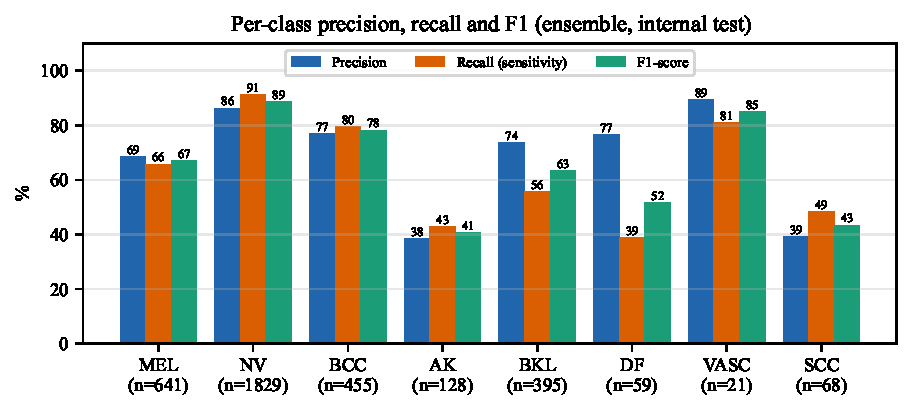
\includegraphics[width=\linewidth]{figures/fig_prf_per_class.pdf}
\caption{Precision, recall, and F1 for each class (ensemble, internal test).}
\end{figure}

\begin{table}[H]
\centering
\caption{External test set (PAD-UFES-20, 2{,}298 phone photos, 6 classes).}
\renewcommand{\arraystretch}{1.2}
\small
\begin{tabular}{@{}l c c c c c@{}}
\toprule
\textbf{Model} & \textbf{Accuracy} & \textbf{Precision} & \textbf{Recall (=BA)} & \textbf{F1} & \textbf{Cancer AUC} \\
\midrule
EfficientNetV2-S & 33.68\% & 34.75\% & 39.74\% & 28.50\% & 0.833 \\
ConvNeXt-T & 34.73\% & 33.82\% & 38.22\% & 28.64\% & 0.844 \\
Swin-T & 35.34\% & 35.34\% & 41.50\% & 30.03\% & 0.844 \\
\textbf{Ensemble (equal)} & \textbf{37.25\%} & \textbf{37.05\%} & \textbf{41.89\%} & \textbf{30.74\%} & \textbf{0.873} \\
\bottomrule
\end{tabular}
\end{table}

\inpaper{Table IV (internal, with precision), Table V (per-class
precision/recall/F1), Table VII (external), Fig.~5 (bar charts),
Fig.~7 (ROC), Table VI (ablation: 1 vs.\ 2 vs.\ 3 models).}

% =====================================================================
\section{Example Images from the Test Set}
\subsection*{(a) Correct predictions --- one per class}
\begin{figure}[H]
\centering
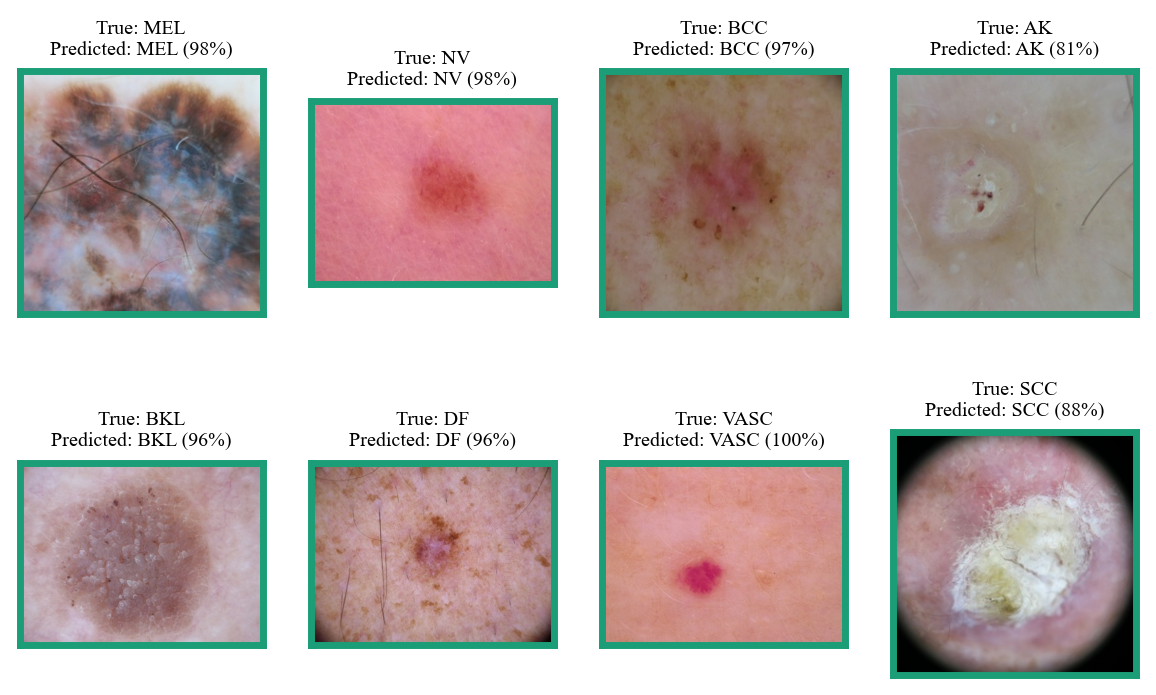
\includegraphics[width=0.92\linewidth]{figures/fig_examples_correct.png}
\caption{Real test images (never seen in training). Green frame = correct. The percentage is the ensemble's confidence.}
\end{figure}

\subsection*{(b) Why combining models helps (our USP)}
\begin{figure}[H]
\centering
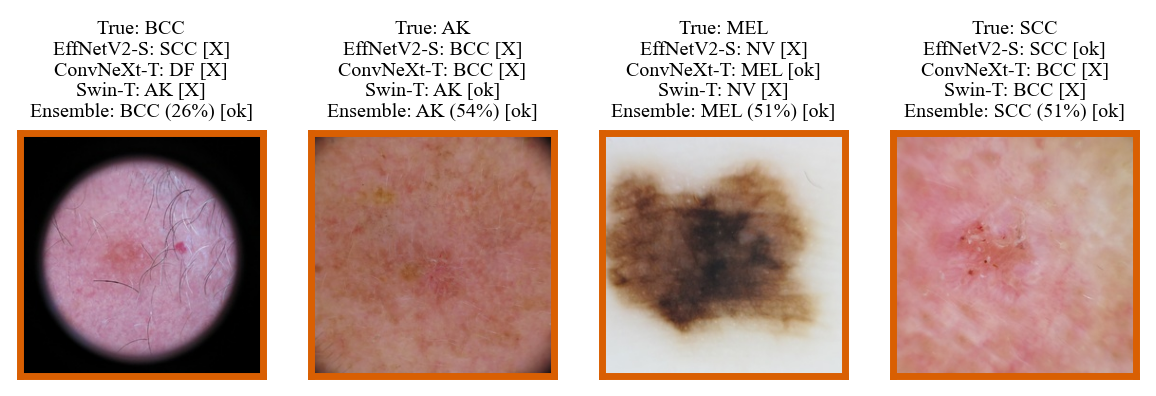
\includegraphics[width=\linewidth]{figures/fig_examples_usp.png}
\caption{Cases where one or more single models were wrong but the ensemble was right. In the first image all three models were wrong individually, yet the average of their probabilities picked the correct class. In the internal test set this happened 556 times; the opposite (ensemble wrong although at least one model was right) happened 290 times.}
\end{figure}

\subsection*{(c) Typical mistakes}
\begin{figure}[H]
\centering
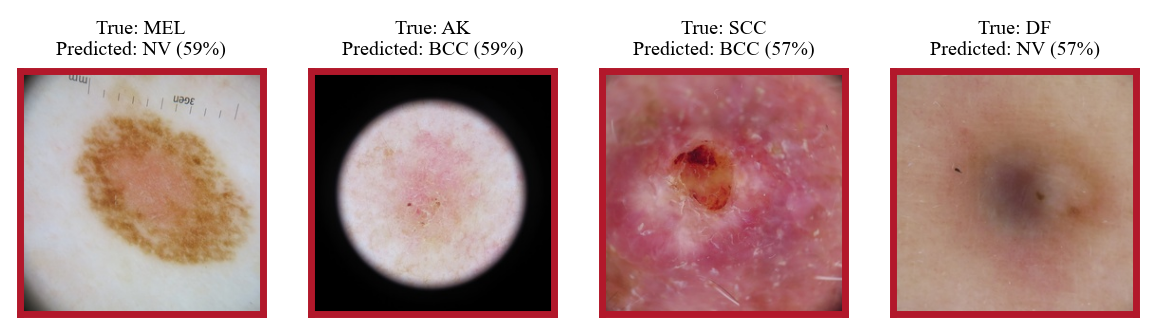
\includegraphics[width=\linewidth]{figures/fig_examples_errors.png}
\caption{Red frame = wrong. These are the most common confusions in the confusion matrix: melanoma vs.\ nevus, AK/SCC vs.\ BCC, dermatofibroma vs.\ nevus. They are also hard for doctors.}
\end{figure}

\subsection*{(d) Phone photos (PAD-UFES-20)}
\begin{figure}[H]
\centering
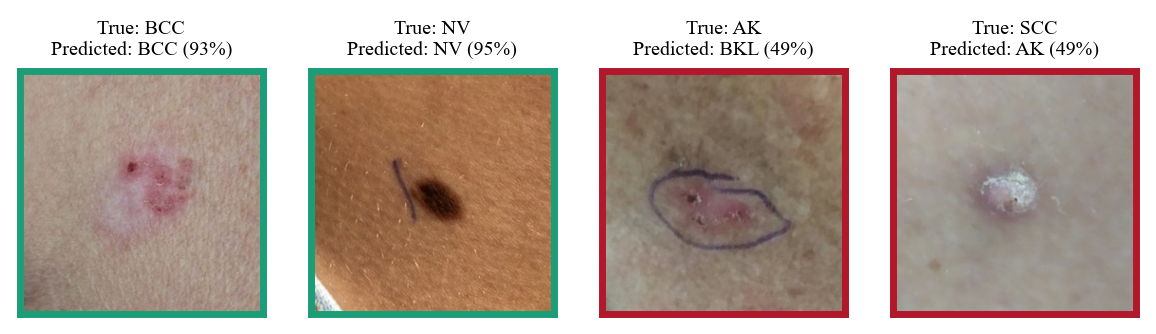
\includegraphics[width=\linewidth]{figures/fig_examples_external.png}
\caption{External test. Phone photos look different from dermoscope close-ups, which is why accuracy drops to 37\%.}
\end{figure}

% =====================================================================
\section{Where Everything Is in the Paper}
\begin{tabularx}{\linewidth}{@{}L{5.0cm} Y@{}}
\toprule
\textbf{Item} & \textbf{Location in \texttt{sc\_two\_column.pdf}} \\
\midrule
Datasets used and split sizes & Section III; Table II (rows marked ``Used''); Section V-A \\
Which models, pre-trained weights & Section IV-D (Hybrid backbone ensemble) \\
How we trained (steps, settings, time) & Section IV-F (focal loss, Eq.~3), IV-I (training procedure), Algorithm 1, Table III \\
How models are combined & Section IV-G, Eq.~(4) \\
How accuracy, precision, recall, F1 are calculated & Section V-B, Eqs.~(6)--(8) \\
Training graph & Fig.~4 (Section VI-A) \\
Accuracy and precision of every model & Table IV and Fig.~5(a) (Section VI-B) \\
Confusion matrix & Fig.~6 (Section VI-C) \\
Per-class precision / recall / F1 & Table V (Section VI-C) \\
ROC curve & Fig.~7 (Section VI-C) \\
USP proof (1 vs.\ 2 vs.\ 3 models) & Table VI (Section VI-D) \\
External phone-photo results & Table VII and Fig.~5(b) (Section VI-E) \\
Skin-type results & Section VI-F \\
Final accuracy and conclusion & Abstract and Section IX \\
\bottomrule
\end{tabularx}

\keybox{\textbf{What to tell your teacher (30 seconds):} ``We trained three
models --- two CNNs and one transformer --- on the same 18{,}076 ISIC~2019
images, chose the best epoch on 3{,}659 validation images, and averaged
their predictions. On 3{,}596 unseen test images the combined model was
right 2{,}803 times, which is 77.95\% accuracy, with 68.67\% precision,
62.99\% balanced accuracy, and an AUC of 0.950. It found 95.4\% of the
cancers. The confusion matrix in Fig.~6 shows where it makes mistakes,
mainly melanoma versus nevus. Combining the models beat every single
model and every pair, which is our USP. On phone photos it drops to 37\%,
which shows what we need to improve next.''}

\end{document}
